% LaTeX source package generated from the project manuscript.
% Current positioning: Methods of Information in Medicine health-informatics method study.
\documentclass[pdflatex,sn-nature]{sn-jnl}

\usepackage{graphicx}
\usepackage{booktabs}
\usepackage{longtable}
\usepackage{array}
\usepackage{url}
\usepackage{amsmath,amssymb}
\usepackage{setspace}
\usepackage{lineno}

\graphicspath{{figures/}}
\makeatletter
\newcommand{\inlinefigurecaption}[2]{%
  \begingroup
  \def\@captype{figure}%
  \caption{#2}%
  \label{#1}%
  \endgroup
}
\makeatother
\raggedbottom

\begin{document}
\doublespacing
\linenumbers

\title[Self-supervised CTG representation]{Self-supervised cardiotocography trajectory representation for calibrated neonatal risk enrichment: an open-data health informatics method study}

\author[1]{\fnm{Xiaoqian} \sur{Gui}}\email{1543678562@qq.com}
\equalcont{These authors contributed equally to this work.}

\author[2]{\fnm{Kaisi} \sur{Zhu}}\email{chzks6768@163.com}
\equalcont{These authors contributed equally to this work.}

\author[3]{\fnm{Ziyi} \sur{Jiang}}\email{15821623673@163.com}
\equalcont{These authors contributed equally to this work.}

\author*[4]{\fnm{Feifan} \sur{Lu}}\email{luff94@163.com}

\affil[1]{\orgdiv{Changhai Center for Simulation, Learning and Innovation}, \orgname{Changhai Hospital, Naval Medical University}, \orgaddress{\city{Shanghai}, \postcode{200433}, \country{China}}}

\affil[2]{\orgdiv{Department of Anesthesiology}, \orgname{Changhai Hospital, Naval Medical University}, \orgaddress{\city{Shanghai}, \postcode{200433}, \country{China}}}

\affil[3]{\orgdiv{Department of General Internal Medicine}, \orgname{The 929th Hospital, Affiliated with Changhai Hospital, Naval Medical University}, \orgaddress{\country{China}}}

\affil*[4]{\orgdiv{Department of Obstetrics and Gynecology}, \orgname{Changhai Hospital, Naval Medical University}, \orgaddress{\city{Shanghai}, \postcode{200433}, \country{China}}}

\abstract{\textbf{Background:} Intrapartum cardiotocography (CTG) produces long fetal heart rate (FHR) and uterine contraction (UC) trajectories, but clinical decision support often relies on static summaries or subjective pattern recognition.
\textbf{Objectives:} To evaluate whether an open-data health informatics workflow based on self-supervised CTG trajectory representation can support interpretable neonatal risk enrichment, recalibration and explicit domain-shift assessment.
\textbf{Methods:} We used CTU-UHB/CTU-CHB as the primary open raw-signal cohort and CTGDL-FHRMA for external representation analysis. The binary neonatal-risk endpoint was umbilical artery pH $<$7.15 or 5-minute Apgar score $<$7. CTU-UHB records were split at the record level into 386 training and 166 held-out test records. A compact PatchTST-style transformer encoder was trained on training-record FHR/UC windows only, with outcome labels withheld from self-supervised learning. Classical signal features, self-supervised learning (SSL) embeddings, dynamic phenotypes and combined models were assessed using bootstrap validation, recalibration, decision-curve analysis, development-only model-selection sensitivity, SSL dimensionality sensitivity and pH-threshold outcome sensitivity.
\textbf{Results:} Held-out event prevalence was 20.48\%. Signal-only features achieved an AUPRC of 0.3366 (95\% CI 0.2173--0.4941). Adding SSL embeddings increased AUPRC to 0.4432 (95\% CI 0.2974--0.5891), with a bootstrap AUPRC difference of 0.0978 (95\% CI 0.0148--0.1864). The manuscript-candidate signal-plus-SSL-plus-signal-phenotype model achieved AUROC 0.6560 (95\% CI 0.5490--0.7577) and AUPRC 0.4324 (95\% CI 0.2867--0.5877). A development-only model-selection sensitivity selected a smaller configuration with held-out AUPRC 0.3872. SSL PCA models using 10 and 20 components achieved AUPRCs of 0.4241 and 0.4256. Cross-fitted Platt recalibration improved Brier score from 0.2516 to 0.1524 and expected calibration error from 0.2629 to 0.0248. CTGDL-FHRMA showed substantial representation domain shift, with CTU-versus-CTGDL domain AUROC 0.9088.
\textbf{Conclusions:} Open-data CTG representation learning can support interpretable, calibration-aware neonatal risk enrichment as a reproducible medical informatics method. The current study does not establish external outcome validity or clinical deployability.}

\keywords{medical informatics, cardiotocography, machine learning, clinical decision support, calibration}

\maketitle

\section{Introduction}

Intrapartum CTG monitoring is widely used to assess fetal status during labour, but its clinical value and interpretation remain contested because visual assessment has limited positive predictive value and substantial observer variability \cite{alfirevic2017,figo2015,nichd2008,francis2024}. The clinical decision problem is not merely whether an algorithm can assign a label after delivery. During labour, CTG interpretation may influence closer surveillance, escalation, fetal blood sampling where available, operative delivery or reassurance. A useful informatics model should therefore help enrich risk and explain signal patterns without replacing obstetric judgement. The raw CTG signal is inherently dynamic: FHR and UC traces record how the fetus responds to contractions and changing intrapartum stress over time. In practice, however, this temporal information is often compressed into static summary features, categorical rule systems or visual interpretation. Such compression can support standardisation, but it may also discard trajectory structure that is relevant for decision-oriented risk enrichment and phenotype discovery \cite{mendis2023}.

Self-supervised time-series models provide a possible route from raw physiological trajectories to reusable representations, consistent with the broader foundation-model direction in medicine and with recent transformer-based time-series representation learning \cite{moor2023,zerveas2021,nie2023,yue2022,goswami2024moment}. Recent open-source time-series methods converge on design principles that are well matched to CTG. Patch-level tokenisation can reduce long FHR/UC windows to tractable temporal tokens while preserving local morphology. Random, block, mixed and channel-level masking strategies can expose the encoder to signal loss, temporal corruption and channel-specific degradation, all of which resemble practical CTG artefact and monitoring interruptions. Masked reconstruction then forces the model to recover missing trajectory structure, whereas contrastive objectives encourage embeddings from augmented views of the same underlying record to remain close \cite{nie2023,yue2022,zhang2022tfc}. For obstetric CTG, however, the relevant question is not simply whether a deep model can predict an adverse neonatal label. A credible workflow also has to show that learned representations add information beyond classical signal summaries, that dynamic phenotypes remain clinically interpretable, that absolute risks can be recalibrated, and that external public data are used within their legitimate outcome-label boundaries \cite{tripodai2024,vanCalster2019,vickers2006}. These requirements are especially important for open-data studies, where external datasets may support representation transport or domain-shift assessment without supporting external clinical outcome validation.

Large supervised CTG interpretation studies define a complementary benchmark. In a nationwide multicentre study, Park et al. used 22,522 deliveries from 14 hospitals and 519,800 person-minutes of CTG to train an SE-ResNet50-based normal-versus-abnormal CTG classifier, reporting internal AUROC/PRC of 0.880/0.625 and three external AUROCs of 0.862, 0.895 and 0.862 \cite{park2025nationwide}. That work addresses high-performance supervised abnormal-pattern classification with expert interval labels. The present work addresses a different open-data problem: whether raw FHR/UC trajectories can yield reusable self-supervised representations, clinically inspectable phenotypes, calibrated neonatal-risk enrichment and honest domain-shift assessment when large proprietary annotated datasets are unavailable. This methodological boundary has become more important because CTG-specific foundation-model preprints have begun to report strong CTU-UHB prediction performance after large-scale self-supervised pretraining and multi-view learning \cite{fridman2026ctgfoundation,prismctg2026}. Rather than presenting another claim of deployable fetal-stress prediction, we developed an open-data CTG decision-modelling workflow using CTU-UHB/CTU-CHB as the primary raw-signal cohort and CTGDL-FHRMA as an external representation-validation resource \cite{goldberger2000,chudacek2014,ctuuhb,ctgdl}. We trained a compact PatchTST-style masked transformer encoder on FHR and UC windows, derived both signal-based and SSL-based phenotypes, and evaluated neonatal risk enrichment using a fixed record-level split. The analysis combined bootstrap confidence intervals, permutation-based explanation, missingness sensitivity, cross-fitted recalibration, decision curve analysis and external domain-shift assessment. This design was intended to test whether self-supervised CTG representations can support a bounded, reproducible and clinically legible phenotyping-and-calibration workflow rather than to claim an autonomous clinical risk calculator.

\section{Results}

\subsection{Open CTG data defined a leakage-aware phenotyping workflow}

To establish the analysis frame, we used CTU-UHB/CTU-CHB as the primary raw-signal cohort and retained CTGDL-FHRMA for external representation validation. CTU-UHB records were split at the record level into 386 training records and 166 held-out test records, before any downstream window-level modelling. This design reduced leakage between overlapping windows from the same CTG record and approximated a future-record evaluation setting, which is more relevant to decision modelling than random window-level splitting. The resulting workflow linked raw FHR/UC signals to dynamic representations, phenotypes, risk prediction, recalibration and external domain-shift analysis (Fig.~\ref{fig:study_design}).

\subsection{Self-supervised representations improved risk enrichment beyond signal summaries}

To test whether learned trajectory representations added value beyond classical CTG summaries, we compared signal-only, SSL-augmented and phenotype-augmented models in the held-out CTU-UHB test set. The neonatal-risk endpoint occurred in 79 of 386 training records (20.47\%) and 34 of 166 held-out test records (20.48\%). Signal-only features achieved an AUPRC of 0.3366 (95\% CI 0.2173--0.4941), corresponding to 1.64-fold enrichment over the held-out event prevalence. Adding transformer SSL embeddings increased AUPRC to 0.4432 (95\% CI 0.2974--0.5891), corresponding to 2.16-fold enrichment, with a bootstrap AUPRC difference of 0.0978 (95\% CI 0.0148--0.1864) versus signal-only features. The manuscript-candidate signal-plus-SSL-plus-signal-phenotype model achieved an AUROC of 0.6560 (95\% CI 0.5490--0.7577) and an AUPRC of 0.4324 (95\% CI 0.2867--0.5877), corresponding to 2.11-fold enrichment over prevalence. Its AUPRC difference versus signal-only features was 0.0891 (95\% CI 0.0073--0.1766). Because the compact transformer ranking used held-out AUPRC for method exploration, we performed an additional development-only model-selection sensitivity analysis within the original training records. In that analysis, a 75\%/25\% stratified split of the training records selected the smaller p80-d48-l2 mixed-masking signal-plus-SSL-plus-signal-phenotype configuration; when then fitted on all original training records and evaluated once in the held-out test set, this development-selected configuration achieved an AUROC of 0.6348, AUPRC of 0.3872 and Brier score of 0.2542. We therefore interpret the held-out-ranked transformer comparison as exploratory and the overall result as evidence of risk enrichment rather than a locked external model-selection result (Supplementary Table~\ref{tab:supp_index}). This pattern is important for clinical decision relevance because a low-prevalence neonatal risk task is often used for enrichment or triage rather than definitive diagnosis. AUPRC directly reflects how well high-scoring records concentrate true adverse outcomes among records selected for attention, whereas AUROC can remain insensitive to clinically relevant changes in the high-risk tail. By contrast, AUROC and Brier-score differences crossed zero, indicating that the most stable gain was risk enrichment under class imbalance rather than global discrimination or raw calibration (Fig.~\ref{fig:model_validation}A--D; Fig.~\ref{fig:model_selection_sensitivity}A,B).

Permutation analysis supported a mixed clinical and representation-based signal. In the signal-plus-SSL model, the positive AUPRC importance sum was 0.4874 for clinical signal features and 2.6003 for SSL embedding dimensions. Mean positive AUPRC importance per feature was similar across the two families (0.0406 and 0.0406, respectively), suggesting that the observed gain was distributed across multiple embedding dimensions rather than driven by a single latent variable (Fig.~\ref{fig:model_validation}F; Fig.~\ref{fig:model_selection_sensitivity}D).

Because FHR missingness contributed to prediction, models were rerun after excluding FHR and UC missingness fractions. Without missingness features, signal plus SSL achieved an AUPRC of 0.4284 (95\% CI 0.2800--0.5823), and the final model achieved an AUPRC of 0.4319 (95\% CI 0.2858--0.5855). The no-missingness AUPRC difference for the final model versus signal-only features was 0.0489 (95\% CI -0.0308--0.1309). These results show directionally retained enrichment, but they do not establish a statistically secure missingness-independent gain (Fig.~\ref{fig:model_validation}E). To address the high-dimensionality concern, we repeated the final model using principal components of the SSL embeddings fitted within the training records. A 10-component SSL PCA representation explained 95.67\% of training embedding variance and achieved an AUPRC of 0.4241 with 23 predictors before one-hot expansion; a 20-component representation explained 99.53\% of variance and achieved an AUPRC of 0.4256 with 33 predictors. These reduced-dimensional models approached the full 64-dimensional SSL model AUPRC of 0.4324 while increasing the training event-to-predictor ratio from 1.03 to 3.43 and 2.39, respectively (Supplementary Table~\ref{tab:supp_index}).

Outcome-threshold sensitivity analyses supported the same enrichment direction but also illustrated the limits imposed by sparse severe events. For the pH-only endpoint pH $<$7.10, the held-out event prevalence was 11.45\% (19 events), and the final feature set achieved an AUPRC of 0.4870, or 4.25-fold enrichment over prevalence. For pH $<$7.05, the held-out event prevalence was 9.04\% (15 events), and the final feature set achieved an AUPRC of 0.5260, or 5.82-fold enrichment. These analyses were treated as sensitivity checks rather than definitive secondary endpoints because the severe-acidosis event counts were small (Supplementary Table~\ref{tab:supp_index}).

\subsection{Signal phenotypes anchored the latent model in CTG physiology}

To make the modelling output clinically legible, we derived signal-based phenotypes and selected representative prototype records. The four signal-derived phenotypes showed interpretable differences in neonatal risk and CTG signal profiles. Signal phenotype 2 had the highest neonatal risk rate (0.3439), lower mean cord pH (7.1877), higher FHR standard deviation (22.2159) and higher deceleration-proxy burden (3530.4777). This profile is consistent with a subgroup in which fetal heart rate responses to uterine activity are more unstable and deceleration-prone, although the retrospective data do not prove a causal fetal-distress mechanism. Signal phenotype 4 had the lowest neonatal risk rate (0.1048). Prototype records illustrated the paired FHR and UC patterns underlying each phenotype (Fig.~\ref{fig:phenotypes}). These results positioned signal phenotypes as the main clinical interpretation layer for the SSL-enhanced model: the latent encoder contributed risk information, while phenotype prototypes translated part of that information into recognizable CTG trajectory patterns.

\subsection{Platt recalibration improved absolute risk estimates and threshold behavior}

Because risk enrichment alone does not make a clinically usable probability, we next evaluated calibration and threshold behaviour. Raw deep-model scores should not be interpreted as absolute neonatal risk, particularly when the development cohort, outcome definition and signal quality differ from future clinical settings. Raw predictions from the final signal-plus-SSL-plus-signal-phenotype model were poorly calibrated. The raw Brier score was 0.2516 (95\% CI 0.2150--0.2863), and the raw expected calibration error was 0.2629 (95\% CI 0.2044--0.3313). Cross-fitted Platt recalibration improved the Brier score to 0.1524 (95\% CI 0.1223--0.1863). The held-out expected calibration error decreased to 0.0248; because expected calibration error is bin-dependent and bootstrap samples altered bin composition, the bootstrap mean was 0.0624 (95\% CI 0.0261--0.1084). Bootstrap differences for Platt minus raw predictions were -0.0991 for Brier score (95\% CI -0.1410 to -0.0566) and -0.2052 for expected calibration error (95\% CI -0.2554 to -0.1294). In the 0.10--0.30 threshold range, mean net benefit increased from 0.0320 for raw predictions to 0.0513 after Platt recalibration. Isotonic recalibration improved some calibration metrics but reduced AUPRC, so it was treated as exploratory (Fig.~\ref{fig:calibration_dca}). These findings make recalibration a necessary decision-modelling step rather than a cosmetic post-processing analysis.

\subsection{CTGDL-FHRMA showed representation transport with substantial domain shift}

Finally, we examined whether the trained representation could be projected onto an external open CTG resource. External CTGDL-FHRMA analysis included 135 records and was compared with 552 CTU-UHB records in the transformer embedding space. The first two principal components explained 0.5092 of embedding variance. A CTU-versus-CTGDL domain classifier achieved an AUROC of 0.9088, indicating substantial domain shift. CTGDL-FHRMA records were assigned across CTU-derived SSL phenotypes, with most assigned to phenotypes 1 and 3. We treated this as a prespecified boundary rather than a failed external validation exercise: because CTGDL-FHRMA did not provide the same neonatal outcome structure used in CTU-UHB, forcing an external outcome comparison would risk a misleading estimate of clinical generalisability. These analyses therefore support external representation transport and domain-shift validation, not external clinical outcome validation (Fig.~\ref{fig:external}). Transformer model-selection and SSL phenotype sensitivity panels are provided as supplementary evidence for the final figure package (Fig.~\ref{fig:model_selection_sensitivity}).

\section{Discussion}

This open-data CTG study demonstrates a bounded use case for self-supervised intrapartum trajectory modelling in health informatics. The main contribution is not a stand-alone clinical predictor, but a reproducible workflow that links masked time-series representations, clinically interpretable signal phenotypes, bootstrap validation, recalibration and external domain-shift assessment. This positioning is aligned with recent reviews emphasizing that automated CTG models require stronger generalisability, standardised outcome definitions and clearer translation pathways before clinical deployment \cite{mendis2023,francis2024}. In a decision-support context, the value of such a workflow lies in risk enrichment, signal explanation and calibration discipline rather than in replacing real-time obstetric judgement. The most consistent performance gain was observed for AUPRC, which matches the class-imbalanced neonatal risk setting \cite{davis2006}. The evidence did not support a stable AUROC gain, and raw probabilities were poorly calibrated before recalibration \cite{vanCalster2019}.

Compared with the nationwide supervised interpretation model reported by Park et al. \cite{park2025nationwide}, our dataset and validation scale are modest, and this manuscript should not be read as competing with multicentre external validation of expert-labelled abnormal CTG interpretation. Its contribution is complementary: a reproducible open-data method layer for self-supervised trajectory representation, phenotype prototypes, calibration-aware risk enrichment, decision-curve analysis and explicit representation-domain assessment.

The AI contribution should therefore be interpreted as a transparent representation-learning design rather than as a large-scale foundation model. Patch tokenisation addressed the practical problem that 10-minute two-channel CTG windows are too long to model efficiently as individual time points, while still retaining local FHR and UC morphology. Masking-strategy experiments made the pretext task closer to CTG practice, where signal dropout, blocked artefact and channel-specific degradation are common; the final held-out model used channel masking after the compact sweep, while mixed and block masking were retained as sensitivity configurations. Masked reconstruction encouraged recovery of missing trajectory information, and the NT-Xent objective encouraged two augmented views of the same physiological record to occupy a consistent representation space. Phenotype clustering then converted part of this latent space into a form that can be inspected by clinicians through prototypes and signal summaries. These components are established in contemporary time-series SSL systems \cite{nie2023,yue2022,zhang2022tfc,goswami2024moment}. Together, they make the work methodologically stronger than a conventional CNN or LSTM CTG classifier, but it remains smaller than recent CTG-specific foundation-model efforts that use larger unlabelled corpora, multi-view objectives, pretrained weights or broader downstream benchmarks \cite{fridman2026ctgfoundation,prismctg2026}. Our differentiating claim is consequently clinical and methodological integration: dynamic phenotype discovery, leakage-aware validation, calibration, decision-curve analysis, missingness sensitivity and external representation-domain assessment.

\subsection{Clinical decision-support implications}

The intended clinical informatics role is risk enrichment and information organization, not autonomous diagnosis. A calibrated trajectory-representation workflow could help investigators or future decision-support systems summarize long CTG records into inspectable phenotypes, identify records that warrant closer review, and communicate uncertainty on a probability scale after local recalibration. In the current study, these implications remain methodological because the model has not undergone institutionally external outcome validation or prospective workflow evaluation.

The phenotype analysis provides the main bridge between latent representations and clinical interpretation. Signal phenotype 2 combined higher neonatal risk, lower mean cord pH, greater FHR variability and higher deceleration-proxy burden. This pattern is consistent with an intrapartum subgroup in which fetal cardiovascular responses to uterine activity are more unstable and deceleration-prone, but it should not be read as proof of a single pathophysiological mechanism. The value for decision informatics is that a clinician or investigator can inspect a prototype curve, signal summaries and model risk enrichment together, instead of receiving an opaque latent embedding alone. The workflow therefore separates representation learning from interpretation while allowing both layers to contribute to risk enrichment.

Recalibration materially changed the interpretation of the prediction scores. Cross-fitted Platt scaling improved Brier score and expected calibration error without altering the underlying ranking metrics. This distinction is central for clinical decision relevance. A high uncalibrated deep-model score may be useful for ranking records for attention, but it should not be communicated as an absolute probability of neonatal compromise. Platt recalibration provided a simple way to map the enrichment score onto a more interpretable probability scale under the fixed validation design. In the current sample, isotonic calibration was less attractive because it improved selected calibration summaries while reducing AUPRC.

Several limitations define the scope of these findings. The analysis was retrospective and public-data based. CTGDL-FHRMA was used for representation transport and domain-shift assessment, not for external neonatal outcome validation. This was a deliberate validity decision: outcome definitions, label availability and cohort structure were not sufficiently aligned to support a fair external clinical performance claim. The current external analysis therefore tests representation transportability, not clinical transportability, and it cannot exclude deterioration of clinical performance in another hospital, device environment or outcome-labeling system. The compact transformer sweep was exploratory; although SSL pretraining and supervised fitting respected the record-level split, configuration ranking by held-out AUPRC can overstate the independence of the manuscript-candidate performance estimate. A development-only model-selection sensitivity analysis gave a lower but directionally consistent held-out AUPRC, so future work should use a larger locked train/development/test design, nested resampling or institutionally external validation before any claim of model selection stability. The 64-dimensional SSL embedding model also had a low event-to-predictor ratio; PCA sensitivity analyses showed similar AUPRC with fewer predictors, but the sample size remains too small to support a deployable high-dimensional model. Severe pH-threshold sensitivity analyses were directionally consistent but involved only 15--19 held-out events, so they should be viewed as boundary checks rather than confirmatory secondary endpoints. The model did not use publicly released CTGDL PatchTST weights or PRISM-CTG-style metadata prediction objectives; adding these would require a prespecified benchmark to avoid post hoc method selection. Missingness remained an influential signal-quality and clinical-process marker; after removing missingness features, the SSL benefit was directionally retained but no longer statistically secure. Finally, the model and phenotype definitions require institutionally external and prospective validation before they can be considered for clinical use.

In summary, open CTG data can support self-supervised dynamic phenotyping when the evidence chain includes leakage-aware splitting, baseline comparison, interpretability, calibration and domain-shift analysis. The present results justify further external validation of CTG trajectory phenotypes, but they should not be interpreted as sufficient evidence for clinical deployment.

\section{Methods}

\subsection{Study design and data sources}

This was a retrospective open-data modelling study of intrapartum cardiotocography. CTU-UHB/CTU-CHB was used as the primary raw-signal cohort because it provides FHR, UC, and clinical metadata for intrapartum records \cite{goldberger2000,chudacek2014,ctuuhb}. CTGDL-FHRMA was used for external representation and domain-shift analysis \cite{ctgdl}. UCI Cardiotocography was retained as a feature-level reference resource but was not used as raw-signal outcome validation \cite{uci}. Dataset URLs, access notes, and roles are summarized in Supplementary Table~\ref{tab:supp_index}.

\subsection{Outcome definition}

The primary endpoint was a binary composite neonatal-risk outcome defined at the CTU-UHB record level. A record was coded as positive if available metadata indicated umbilical artery pH $<$7.15 or 5-minute Apgar score $<$7. Records not meeting either criterion were coded as non-events. Neonatal intensive care unit duration and other metadata fields were retained for cohort description where available but were not used in the primary composite endpoint. This definition yielded 113 positive records among 552 CTU-UHB records (20.47\%), including 79 of 386 training records (20.47\%) and 34 of 166 held-out test records (20.48\%).

\subsection{Record split and signal windowing}

Records were split at the record level into training and held-out test sets, following the principle that prediction-model validation must preserve independence between development and evaluation samples \cite{tripod2015,steyerberg2019,tripodai2024}. This split was applied before self-supervised pretraining, phenotype derivation, supervised model fitting, recalibration and held-out validation to prevent leakage between overlapping windows from the same CTG record. FHR and UC signals were converted into fixed-length windows using a target sampling rate of 4 Hz and 10-minute windows. The CTU-UHB corpus contained 7,602 windows, including 5,301 training-record windows and 2,301 held-out test-record windows. Transformer SSL pretraining used only training-record windows and did not use outcome labels. After the encoder was selected and fitted, clean unmasked windows from both splits were encoded for downstream record-level aggregation, with all supervised fitting restricted to the training records and all reported validation metrics computed in the held-out test records.

\subsection{AI model design rationale}

The deep-learning component was selected after reviewing open-source self-supervised time-series methods that could plausibly be reproduced in a public CTG study. PatchTST motivated the use of patch tokens and transformer encoding for long physiological sequences \cite{nie2023}. MOMENT and related time-series foundation-model work motivated masked patch reconstruction as a scalable pretext task \cite{goswami2024moment}. TS2Vec and TF-C motivated contrastive consistency as a complementary representation objective for downstream transfer \cite{yue2022,zhang2022tfc}. The design was adapted to the clinical signal problem rather than imported as a generic architecture: patching reduced long-window complexity, masking strategies approximated signal artefact and channel loss, reconstruction encouraged recovery of trajectory morphology, and contrastive consistency stabilized record-level embeddings across augmented views. We implemented these ingredients locally rather than importing external pretrained CTG weights, because the purpose of this manuscript was to evaluate a transparent, reproducible open-data phenotyping workflow under a fixed CTU-UHB split. The compact transformer sweep should be interpreted as an exploratory method-selection layer. To examine possible held-out selection bias, we added a development-only sensitivity analysis in which candidate configurations were ranked using only an internal split of the original training records, and the selected configuration was then evaluated once in the original held-out test set.

\subsection{Self-supervised time-series representation learning}

A PatchTST-style masked time-series transformer was trained on FHR and UC windows \cite{nie2023}. Each two-channel 10-minute window contained 2,400 time points per channel. The selected manuscript-candidate configuration used non-overlapping patches of length 80, yielding 30 temporal patches per channel and 60 channel-time tokens per window. Each patch was projected to a 64-dimensional latent token, combined with learnable positional and channel embeddings, and passed through a three-layer transformer encoder with four attention heads, feed-forward width four times the model dimension, GELU activation and dropout 0.1. A compact sweep compared patch length, model dimension, number of layers, masking strategy and contrastive weight; the held-out manuscript-candidate used channel masking, mask fraction 0.25 and contrastive objective weight 0.2. During pretraining, two jittered views of each training-record window were independently masked, with Gaussian jitter standard deviation 0.02. The reconstruction term minimized mean squared error only over masked patches, and the contrastive term used an NT-Xent loss with temperature 0.2 over 64-dimensional projected pooled embeddings from the paired views. The total loss was the sum of masked reconstruction loss and the weighted contrastive loss. Candidates in the compact sweep were trained for four epochs with batch size 32 using AdamW, learning rate 0.001, weight decay 0.0001 and gradient-norm clipping at 1.0. A 12-epoch selected-architecture objective trace is shown in Supplementary Fig.~\ref{fig:model_selection_sensitivity}C for training-dynamics inspection; downstream held-out performance was based on the prespecified sweep embeddings. After training, clean unmasked windows were encoded and window embeddings were averaged to record-level SSL representations. This design reflects prior work on transformer time-series representation learning, masked time-series modelling and contrastive transfer learning \cite{zerveas2021,nie2023,yue2022,zhang2022tfc,goswami2024moment}.

\subsection{Dynamic phenotype derivation}

Two complementary phenotype layers were derived. First, classical CTG signal summaries were clustered to produce clinically interpretable signal phenotypes. These summaries included FHR level, FHR variability, low-percentile FHR, UC summaries, FHR-UC correlation, and deceleration-proxy burden. Signal features were median-imputed and standardized using parameters fitted in the training records only. K-means clustering with k=4, random seed 20260521 and 50 initializations was fitted in the training records, and held-out test records were assigned to the nearest learned centroids. The value k=4 was chosen a priori as a compact, clinically inspectable phenotype resolution rather than optimized on outcome performance. Second, record-level SSL embeddings were standardized using training-record parameters and clustered with the same k-means settings to produce representation phenotypes. Prototype records were selected as records closest to phenotype centroids and plotted as paired FHR/UC trajectories.

\subsection{Outcome and prediction models}

Models compared classical signal features, SSL embeddings, signal phenotypes, SSL phenotypes, and combined feature sets. The classical signal model used 12 prespecified record-level features: FHR missing fraction, UC missing fraction, mean FHR, FHR standard deviation, FHR 5th, 50th and 95th percentiles, mean UC, UC standard deviation, UC 95th percentile, FHR-UC correlation and deceleration-proxy count. The SSL-only model used 64 record-level embedding dimensions. The signal-plus-SSL model used 76 numeric variables, and the final signal-plus-SSL-plus-signal-phenotype model used those 76 variables plus one categorical signal-phenotype variable. All supervised prediction models were class-balanced logistic-regression pipelines with median imputation and standardization for numeric predictors, one-hot encoding for categorical phenotype predictors, a liblinear solver, maximum 2,000 iterations and the default L2 penalty. Models were fitted only in the training records and evaluated in the fixed held-out test set. Model comparisons focused on AUROC, AUPRC, and Brier score. AUPRC was prespecified as the main risk-enrichment metric because the neonatal risk outcome was class-imbalanced and because a plausible decision-support use case would be to concentrate attention on a smaller subset of higher-risk CTG records rather than to make a definitive diagnosis from CTG alone \cite{davis2006}.

\subsection{Bootstrap validation and model comparison}

Held-out test-set performance was summarized using observed test-set metrics and 95\% confidence intervals from 2,000 bootstrap resamples. Pairwise model differences were also estimated by bootstrap resampling of the same held-out records. The primary model-comparison emphasis was AUPRC because the neonatal risk outcome was class-imbalanced and because enrichment among high-scoring records is more directly tied to triage-like decision support than average rank separation across all possible thresholds \cite{davis2006,steyerberg2019}.

\subsection{Prediction explanation and missingness sensitivity}

Permutation importance was computed for manuscript-candidate models using AUPRC and AUROC decreases after feature shuffling. Importance values were summarized by feature family and by individual predictor. Because FHR and UC missingness fractions could reflect both signal quality and clinical difficulty of monitoring, sensitivity models were refitted after excluding missingness fractions.

\subsection{Recalibration and decision curve analysis}

Raw held-out predictions were assessed for calibration, because discrimination alone is insufficient for clinical risk prediction \cite{vanCalster2019,steyerberg2019}. Platt and isotonic recalibrators were fitted using five-fold stratified out-of-fold predictions generated within the training records only. For Platt recalibration, a near-unpenalized logistic model was fitted to the logit-transformed out-of-fold probabilities; isotonic recalibration used monotonic isotonic regression with out-of-bounds clipping. The final uncalibrated model was then refitted in all training records, and the learned recalibrators were applied once to the fixed held-out test predictions. Calibration was evaluated using calibration curves, Brier score, calibration intercept, calibration slope, and expected calibration error. Decision curve analysis was used to summarize net benefit across clinically plausible risk thresholds, with emphasis on the 0.10--0.30 threshold range \cite{vickers2006}. This step was treated as part of the decision-modelling pipeline because uncalibrated SSL-enhanced scores can support ranking but cannot be assumed to represent absolute risk.

\subsection{External representation analysis}

The trained transformer encoder was applied to CTGDL-FHRMA windows to obtain external record-level embeddings. CTU-UHB and CTGDL-FHRMA embeddings were compared using principal-component visualization and a domain classifier. CTGDL-FHRMA records were assigned to CTU-derived SSL phenotypes. Because external neonatal outcome labels were not available in a directly harmonized form for the CTU-UHB composite endpoint, this analysis was interpreted as representation and domain-shift validation rather than external outcome validation. This boundary was specified to avoid overstating clinical generalisability from non-equivalent public datasets.

\subsection{Ethical considerations}

This study used publicly available de-identified datasets and did not involve direct contact with human participants, intervention, re-identification or access to identifiable clinical records by the authors. The analysis was therefore treated as secondary analysis of de-identified public data. Dataset-specific ethical approvals and data-use conditions are described by the original data providers.

\section{Availability of data and materials}

The primary CTU-UHB/CTU-CHB dataset is publicly available through PhysioNet \cite{goldberger2000,chudacek2014,ctuuhb}. CTGDL-FHRMA is available through its public Zenodo record with subset-specific access caveats \cite{ctgdl}. UCI Cardiotocography is available through the UCI Machine Learning Repository \cite{uci}. Derived figure source-data tables, supplementary CSV tables, the fixed record-level split and reviewer-sensitivity tables are available in the project repository at \url{https://github.com/Luciky-Leo/ctg-foundation-trajectory} and in the versioned Zenodo archive at \url{https://doi.org/10.5281/zenodo.20376424}.

\section{Code availability}

The analysis code and manuscript source package are available at \url{https://github.com/Luciky-Leo/ctg-foundation-trajectory}. A versioned archival release is available at \url{https://doi.org/10.5281/zenodo.20376424}. The local analysis pipeline is organized under \path{scripts/}. The transformer SSL encoder was trained by \path{scripts/04_models/train_transformer_ssl_encoder.py}; downstream embeddings, phenotypes, validation, recalibration, reviewer-requested sensitivity analyses and figure source-data tables were generated by the remaining scripts in \path{scripts/04_models/} and \path{scripts/05_reports/}. Manuscript figures were generated by \path{scripts/05_reports/build_manuscript_figures.py}. Figure legends, Results text, Methods text, and supplementary tables were generated by \path{scripts/05_reports/build_manuscript_text_and_supplement.py}. The repository includes figure source-data tables, supplementary CSV tables, the fixed record-level split, the TRIPOD+AI checklist and the reviewer-sensitivity table.

\backmatter

\bmhead{Acknowledgements}
The authors acknowledge the maintainers of the public CTU-UHB/CTU-CHB, CTGDL-FHRMA and UCI Cardiotocography resources, and the open-source scientific software communities used in this analysis.

\section*{Declarations}

\bmhead{Funding}
This research received no specific grant from any funding agency in the public, commercial or not-for-profit sectors.

\bmhead{Competing interests}
The authors declare no competing interests.

\bmhead{Ethics approval and consent to participate}
Not applicable. This study used publicly available de-identified datasets.

\bmhead{Consent for publication}
Not applicable.

\bmhead{Author contributions}
X.G., K.Z. and Z.J. contributed equally to source-data verification, literature and clinical-context review, figure and supplementary-material checking, and manuscript revision. F.L. conceived and supervised the study, designed the methodology, implemented the analysis pipeline, curated the public data, performed the formal analyses, generated the figures and source-data tables, and drafted and revised the manuscript. All authors read and approved the final manuscript.

\bmhead{Availability of data and materials}
See the Availability of data and materials section.

\bmhead{Code availability}
See the Code availability section.

\nolinenumbers
\singlespacing
\section{Figures}

\begin{center}
  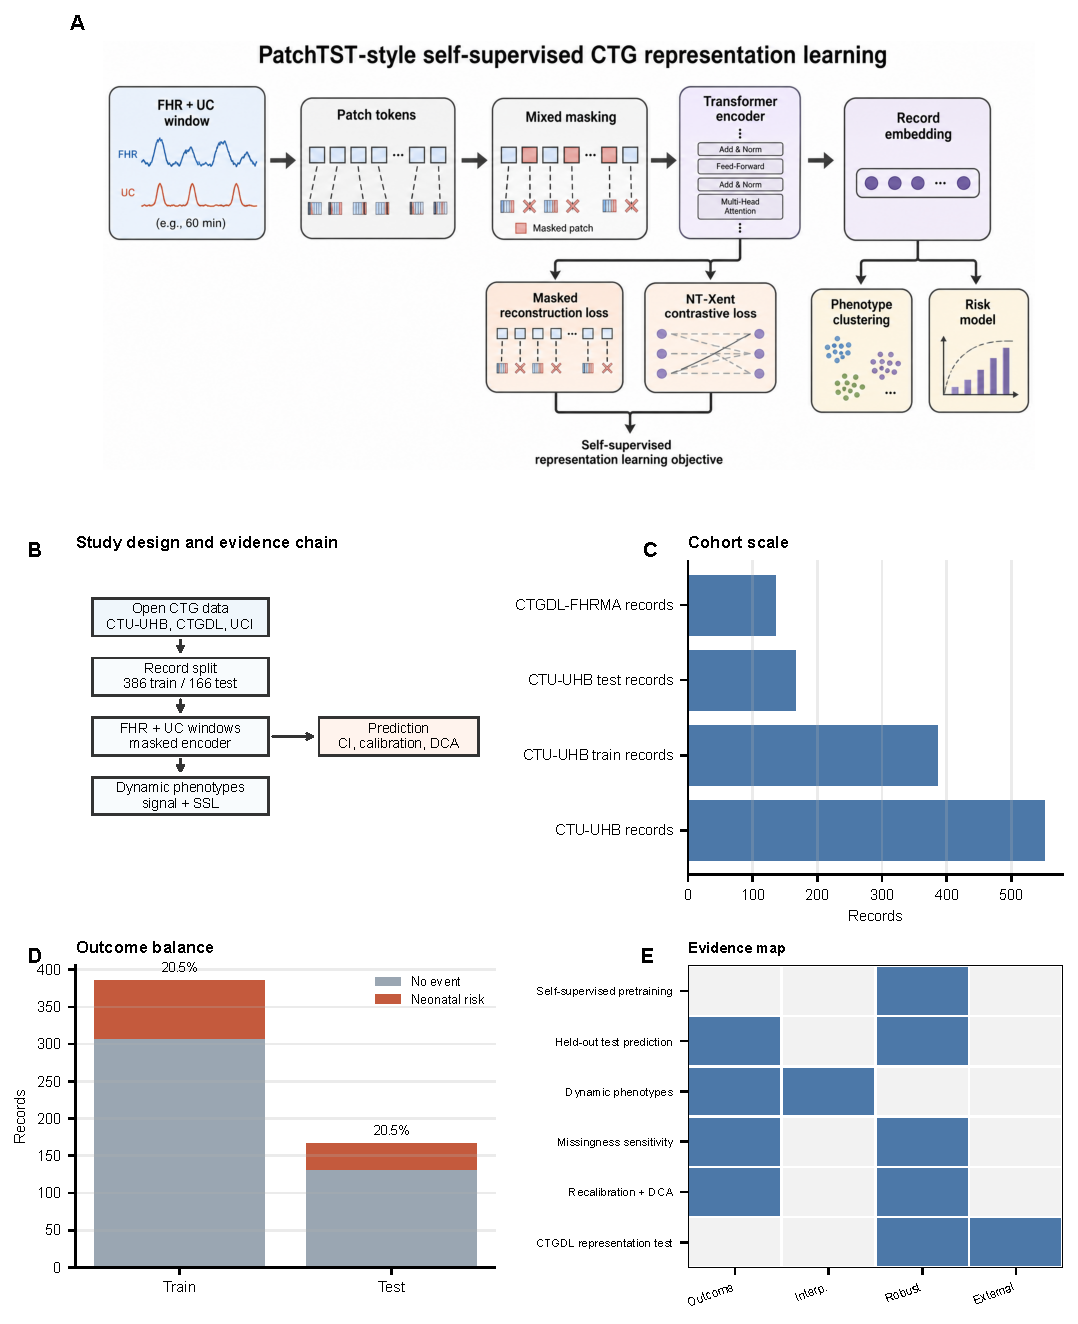
\includegraphics[width=\textwidth,height=0.70\textheight,keepaspectratio]{Figure_1_study_design_pipeline.pdf}
\end{center}
\inlinefigurecaption{fig:study_design}{\textbf{PatchTST-style self-supervised CTG representation learning and evidence chain.}
  Overview of the open-data intrapartum CTG analysis workflow. (A) AI method structure: paired FHR/UC windows were converted into patch tokens, masked by the candidate SSL masking module, encoded by a transformer, trained with masked-patch reconstruction and NT-Xent contrastive consistency, aggregated into record embeddings, and passed to phenotype and risk models. The compact sweep evaluated mixed, block and channel masking; the held-out manuscript-candidate used channel masking. (B) Study design using CTU-UHB/CTU-CHB as the primary raw-signal cohort and CTGDL-FHRMA/UCI Cardiotocography as external representation and feature-level resources. Records were split at the record level into 386 training records and 166 held-out test records. (C) Cohort scale for CTU-UHB training and test records and CTGDL-FHRMA external records. (D) Outcome balance in the record-level training and held-out test split. (E) Evidence map showing which modules support outcome prediction, interpretation, robustness, and external-domain claims.}
\clearpage

\begin{center}
  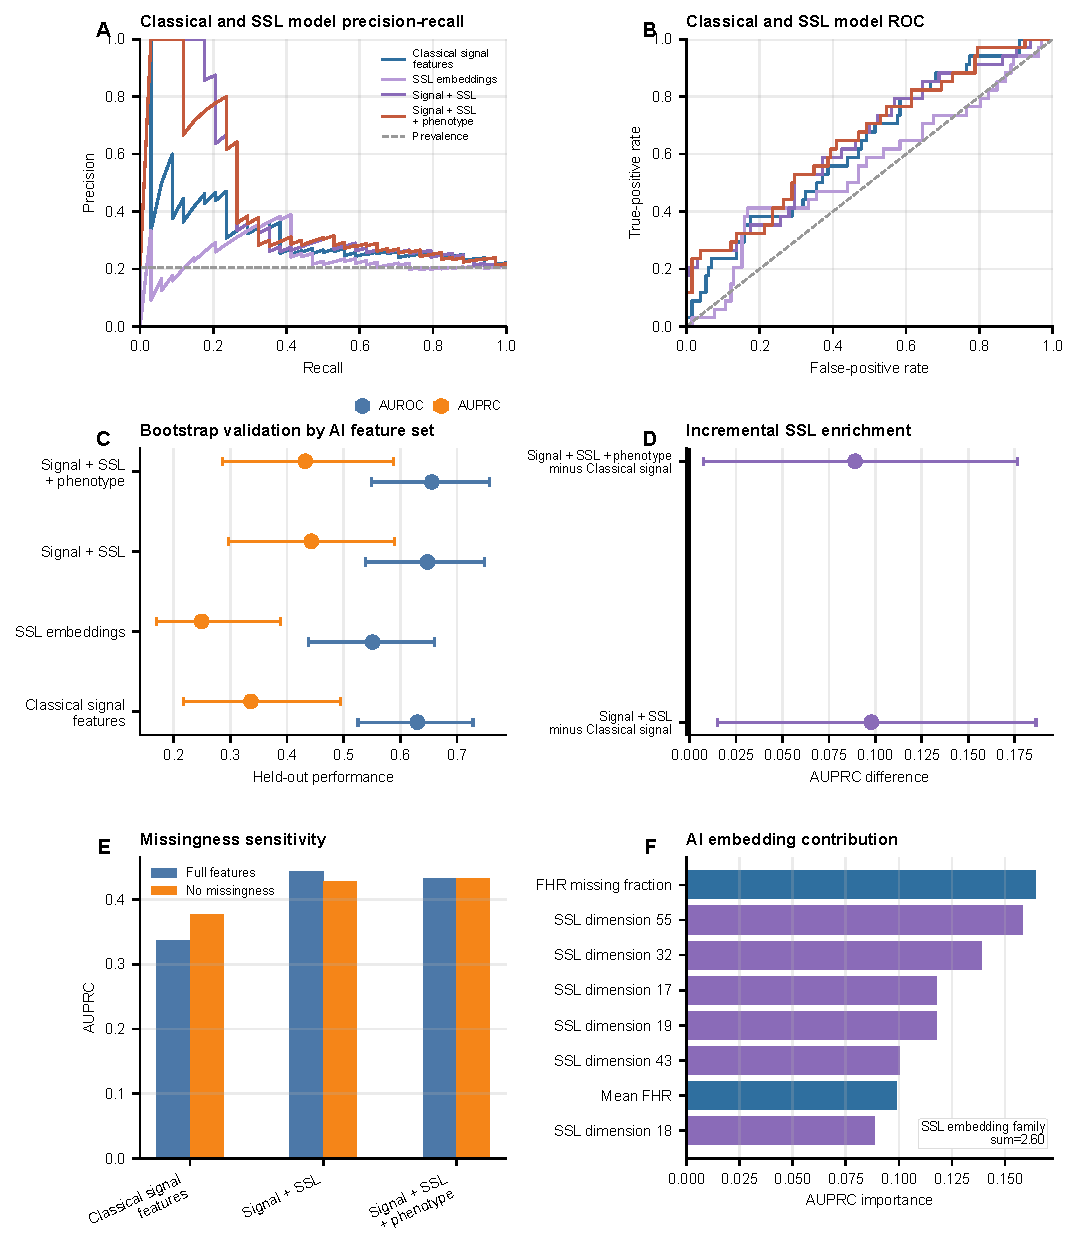
\includegraphics[width=\textwidth,height=0.70\textheight,keepaspectratio]{Figure_2_model_validation_and_explanation.pdf}
\end{center}
\inlinefigurecaption{fig:model_validation}{\textbf{Self-supervised CTG representations improve risk enrichment and contribute measurable AI features.}
  Held-out validation and explanation of neonatal risk prediction models. (A) Precision-recall curves comparing classical signal features, SSL embeddings, signal-plus-SSL, and signal-plus-SSL-plus-phenotype models in the CTU-UHB held-out test set. (B) Receiver-operating-characteristic curves for the same AI feature sets. (C) Bootstrap validation of AUROC and AUPRC; points show observed test-set estimates and whiskers show 95\% bootstrap confidence intervals from 2,000 resamples. (D) Bootstrap AUPRC differences versus classical signal features. (E) Missingness sensitivity after removing FHR and UC missingness fractions from the feature set. (F) AI embedding contribution from AUPRC-based permutation importance in the signal-plus-SSL model; SSL dimensions appear among the highest-ranking predictors and the SSL embedding family contributes substantial aggregate positive importance. SSL, self-supervised learning.}
\clearpage

\begin{center}
  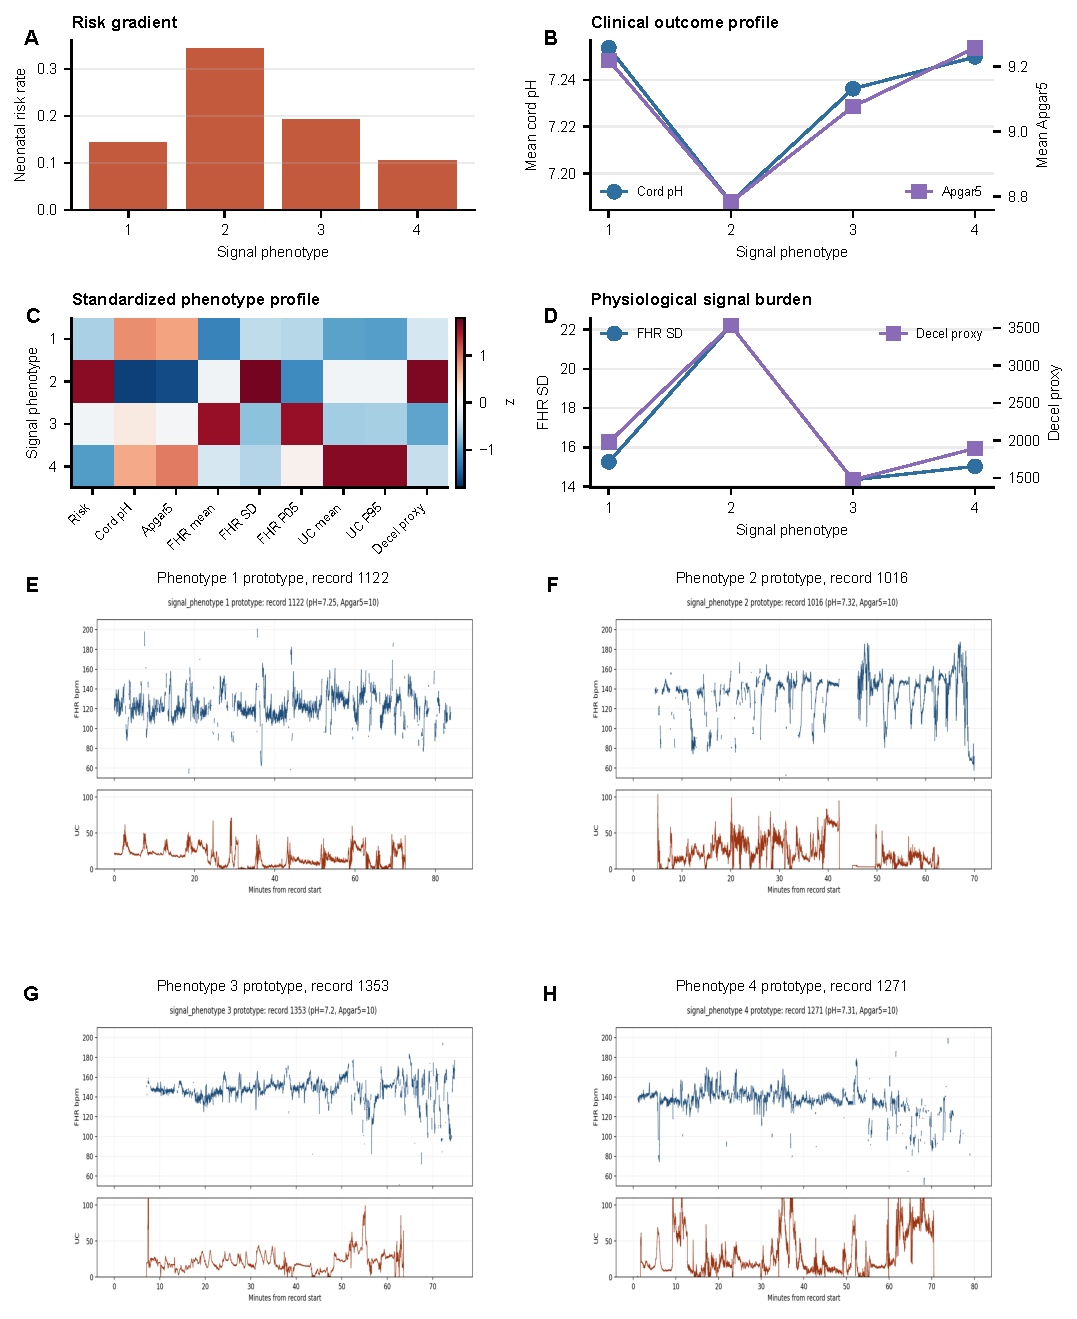
\includegraphics[width=\textwidth,height=0.70\textheight,keepaspectratio]{Figure_3_dynamic_phenotype_prototypes.pdf}
\end{center}
\inlinefigurecaption{fig:phenotypes}{\textbf{Dynamic signal phenotypes provide clinically interpretable CTG prototypes.}
  Signal-derived phenotype structure and representative CTG trajectories. (A) Neonatal risk rates across four signal phenotypes. (B) Mean cord pH and 5-minute Apgar profile across phenotypes. (C) Standardized phenotype profile heatmap summarizing outcome and signal differences. (D) Mean FHR standard deviation and deceleration-proxy burden across signal phenotypes. (E-H) Representative prototype records closest to the phenotype centroids. Phenotype 2 showed the highest neonatal risk rate and the strongest adverse signal profile, including higher FHR variability and deceleration-proxy burden.}
\clearpage

\begin{center}
  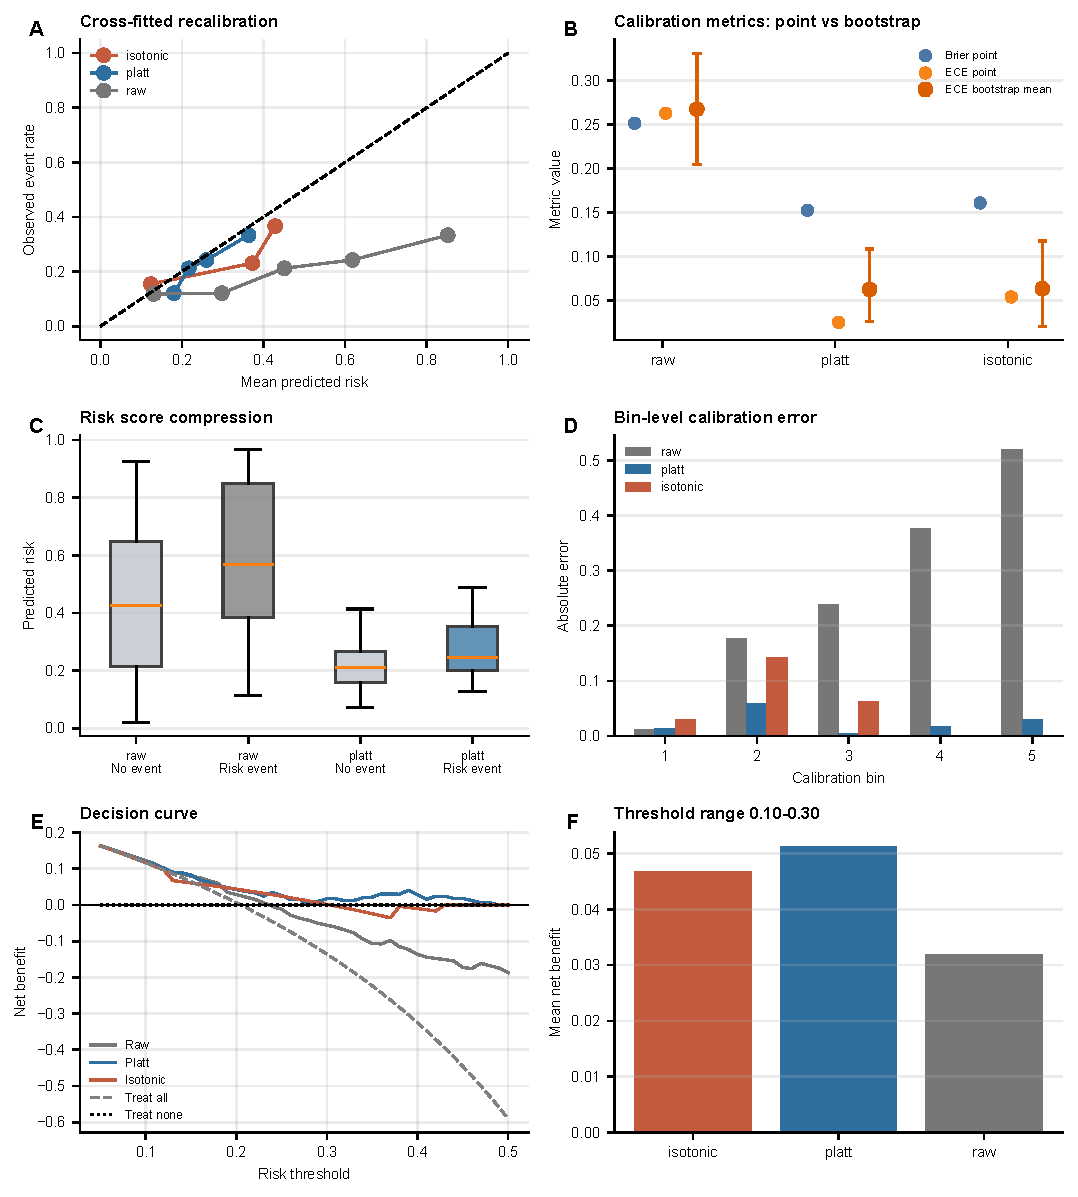
\includegraphics[width=\textwidth,height=0.70\textheight,keepaspectratio]{Figure_4_recalibration_and_clinical_utility.pdf}
\end{center}
\inlinefigurecaption{fig:calibration_dca}{\textbf{Cross-fitted Platt recalibration improves absolute risk calibration and decision-curve behavior.}
  Calibration and clinical utility of the final signal-plus-SSL-plus-signal-phenotype model. (A) Calibration curves for raw, Platt-scaled, and isotonic predictions. Recalibrators were fitted using training-set out-of-fold predictions and evaluated in the held-out test set. (B) Calibration metric panel separating Brier point estimates, ECE point estimates, and bootstrap-mean ECE with 95\% bootstrap confidence intervals; this avoids treating the bin-dependent held-out ECE point estimate as identical to its bootstrap mean. (C) Risk-score distributions before and after Platt recalibration, stratified by observed outcome. (D) Bin-level absolute calibration error. (E) Decision curve analysis across risk thresholds. (F) Mean net benefit in the 0.10--0.30 threshold range. Platt scaling improved calibration while preserving discrimination and AUPRC.}
\clearpage

\section{Supplementary figures}
\setcounter{figure}{0}
\renewcommand{\thefigure}{S\arabic{figure}}
\renewcommand{\theHfigure}{S\arabic{figure}}

\begin{center}
  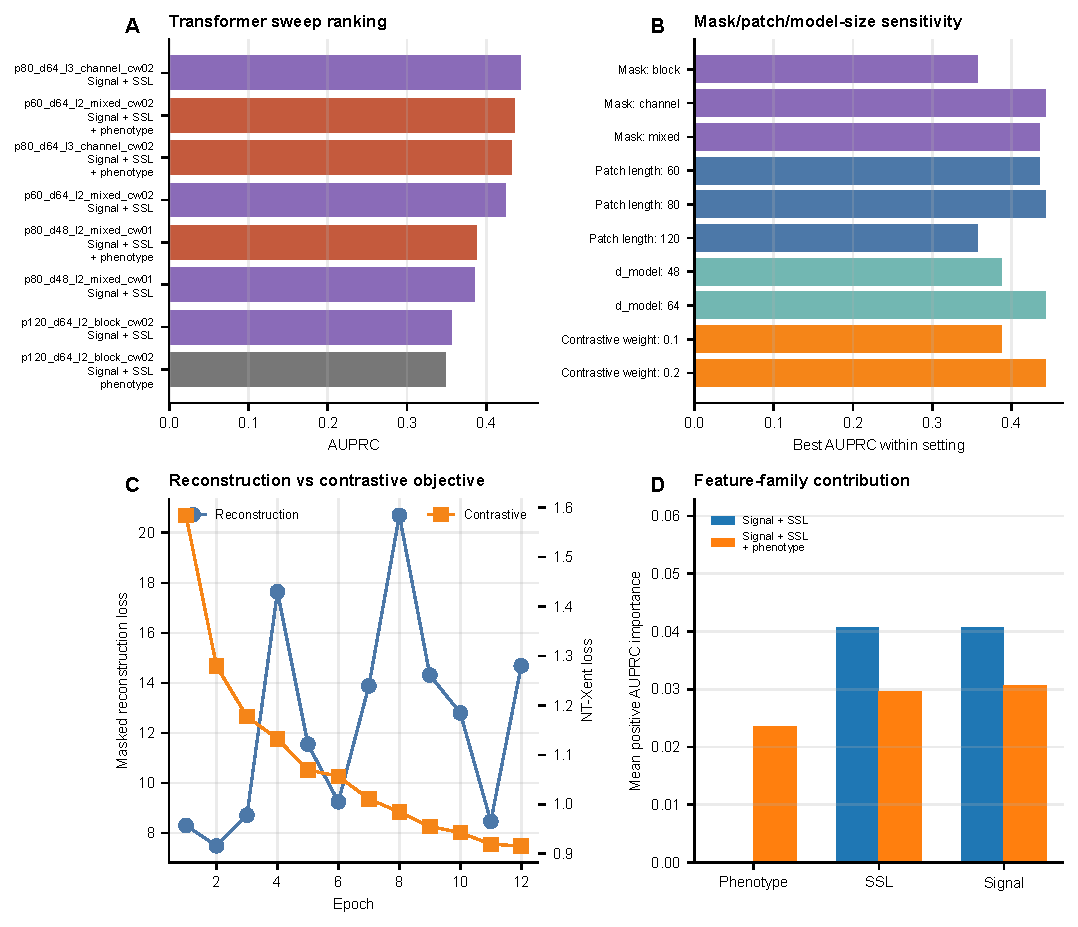
\includegraphics[width=\textwidth,height=0.70\textheight,keepaspectratio]{Supplementary_Figure_S1_model_selection_and_sensitivity.pdf}
\end{center}
\inlinefigurecaption{fig:model_selection_sensitivity}{\textbf{AI model-selection and sensitivity panels for the transformer phenotyping workflow.}
  Supplementary analyses of the self-supervised AI method layer. (A) Exploratory transformer configuration and feature-set combinations ranked by held-out AUPRC. (B) Sensitivity summary across masking strategy, patch length, model dimension and contrastive objective weight, using the best AUPRC observed within each setting. Because these panels use held-out performance for method exploration, they should not be interpreted as a locked independent model-selection experiment. (C) Training-objective trace for a selected-architecture refit, showing masked reconstruction loss and NT-Xent contrastive loss across epochs. (D) Feature-family contribution to AUPRC-based permutation importance for signal-plus-SSL and final phenotype-augmented models.}
\clearpage

\begin{center}
  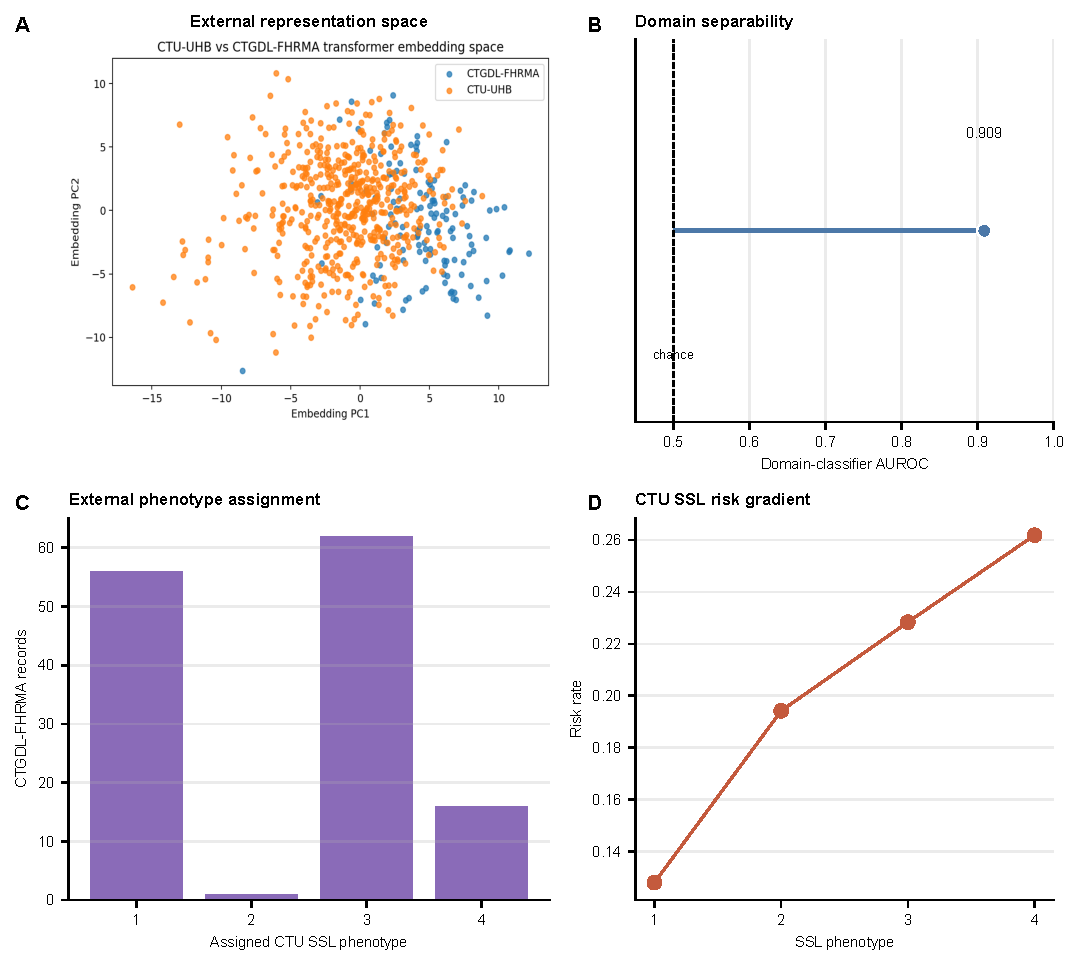
\includegraphics[width=\textwidth,height=0.70\textheight,keepaspectratio]{Supplementary_Figure_S2_external_domain_shift.pdf}
\end{center}
\inlinefigurecaption{fig:external}{\textbf{CTGDL-FHRMA supports external representation and domain-shift validation.}
  External representation analysis using CTGDL-FHRMA records. Because external neonatal outcome labels were not used for CTGDL-FHRMA, this analysis is interpreted as external representation/domain-shift validation rather than external outcome validation. (A) Principal-component visualization of CTU-UHB and CTGDL-FHRMA transformer embeddings. (B) Domain separability quantified by a CTU-versus-CTGDL classifier. (C) CTGDL-FHRMA records assigned to CTU-derived SSL phenotypes. (D) CTU-UHB neonatal risk gradient across SSL phenotypes.}
\clearpage

\section{Supplementary tables}

\begin{longtable}{@{}p{0.20\textwidth}p{0.32\textwidth}p{0.36\textwidth}@{}}
\caption{Supplementary table index. Supplementary CSV files and the combined Excel workbook are included in the \texttt{supplementary\_tables/} directory.}
\label{tab:supp_index}\\
\toprule
Table & File & Description\\
\midrule
\endfirsthead
\toprule
Table & File & Description\\
\midrule
\endhead
Supplementary Table 1 & \path{supplementary_tables/Supplementary_Table_1_datasets_and_cohort_scale.csv} & Dataset sources, cohort scale, record-level split, window counts, and external validation role.\\
Supplementary Table 2 & \path{supplementary_tables/Supplementary_Table_2_model_performance_bootstrap.csv} & Held-out model performance with 2,000-bootstrap confidence intervals.\\
Supplementary Table 3 & \path{supplementary_tables/Supplementary_Table_3_bootstrap_model_differences.csv} & Bootstrap pairwise model differences and zero-crossing flags.\\
Supplementary Table 4 & \path{supplementary_tables/Supplementary_Table_4_dynamic_phenotype_summary_and_prototypes.csv} & Signal and SSL phenotype summaries with representative prototype records.\\
Supplementary Table 5 & \path{supplementary_tables/Supplementary_Table_5_prediction_explainability.csv} & Permutation importance by feature family and top individual predictors.\\
Supplementary Table 6 & \path{supplementary_tables/Supplementary_Table_6_missingness_sensitivity.csv} & Performance and model-difference sensitivity after removing missingness features.\\
Supplementary Table 7 & \path{supplementary_tables/Supplementary_Table_7_recalibration_and_decision_curve.csv} & Cross-fitted recalibration metrics, recalibration differences, and decision curve summaries.\\
Supplementary Table 8 & \path{supplementary_tables/Supplementary_Table_8_external_representation_validation.csv} & CTGDL-FHRMA domain-shift and phenotype-assignment validation.\\
Supplementary Table 9 & \path{supplementary_tables/Supplementary_Table_9_reviewer_sensitivity_analyses.csv} & Reviewer-requested sensitivity analyses for development-only model selection, SSL PCA dimensionality reduction, elastic-net regularization and pH-threshold outcome definitions.\\
Supplementary Table 10 & \path{supplementary_tables/Supplementary_Table_10_TRIPOD_AI_checklist.csv} & TRIPOD+AI reporting checklist mapping for the manuscript.\\
\bottomrule
\end{longtable}

\begin{thebibliography}{99}

\bibitem{alfirevic2017}
Alfirevic, Z., Devane, D., Gyte, G. M. L. \& Cuthbert, A.
Continuous cardiotocography (CTG) as a form of electronic fetal monitoring (EFM) for fetal assessment during labour.
\textit{Cochrane Database Syst. Rev.} \textbf{2017}, CD006066 (2017).
doi:10.1002/14651858.CD006066.pub3.

\bibitem{figo2015}
Ayres-de-Campos, D., Spong, C. Y. \& Chandraharan, E.
FIGO consensus guidelines on intrapartum fetal monitoring: Cardiotocography.
\textit{Int. J. Gynaecol. Obstet.} \textbf{131}, 13--24 (2015).
doi:10.1016/j.ijgo.2015.06.020.

\bibitem{nichd2008}
Macones, G. A., Hankins, G. D. V., Spong, C. Y., Hauth, J. \& Moore, T.
The 2008 National Institute of Child Health and Human Development workshop report on electronic fetal monitoring: update on definitions, interpretation, and research guidelines.
\textit{J. Obstet. Gynecol. Neonatal Nurs.} \textbf{37}, 510--515 (2008).
doi:10.1111/j.1552-6909.2008.00284.x.

\bibitem{mendis2023}
Mendis, L., Palaniswami, M., Brownfoot, F. \& Keenan, E.
Computerised cardiotocography analysis for the automated detection of fetal compromise during labour: a review.
\textit{Bioengineering} \textbf{10}, 1007 (2023).
doi:10.3390/bioengineering10091007.

\bibitem{francis2024}
Francis, F., Luz, S., Wu, H., Stock, S. J. \& Townsend, R.
Machine learning on cardiotocography data to classify fetal outcomes: a scoping review.
\textit{Comput. Biol. Med.} \textbf{172}, 108220 (2024).
doi:10.1016/j.compbiomed.2024.108220.

\bibitem{park2025nationwide}
Park, C. E., Choi, B., Park, R. W. \textit{et al.}
Automated interpretation of cardiotocography using deep learning in a nationwide multicenter study.
\textit{Sci. Rep.} \textbf{15}, 19617 (2025).
doi:10.1038/s41598-025-02849-4.

\bibitem{frasch2021}
Frasch, M. G., Strong, S. B., Nilosek, D., Leaverton, J. \& Schifrin, B. S.
Detection of preventable fetal distress during labor from scanned cardiotocogram tracings using deep learning.
\textit{Front. Pediatr.} \textbf{9}, 736834 (2021).
doi:10.3389/fped.2021.736834.

\bibitem{deepctg2023}
Ben M'Barek, I., Jauvion, G., Vitrou, J., Holmstrom, E., Koskas, M. \& Ceccaldi, P.-F.
DeepCTG 1.0: an interpretable model to detect fetal hypoxia from cardiotocography data during labor and delivery.
\textit{Front. Pediatr.} \textbf{11}, 1190441 (2023).
doi:10.3389/fped.2023.1190441.

\bibitem{goldberger2000}
Goldberger, A. L. \textit{et al.}
PhysioBank, PhysioToolkit, and PhysioNet: components of a new research resource for complex physiologic signals.
\textit{Circulation} \textbf{101}, e215--e220 (2000).
doi:10.1161/01.CIR.101.23.e215.

\bibitem{chudacek2014}
Chudacek, V., Spilka, J., Bursa, M., Janku, P., Hruban, L., Huptych, M. \& Lhotska, L.
Open access intrapartum CTG database.
\textit{BMC Pregnancy Childbirth} \textbf{14}, 16 (2014).
doi:10.1186/1471-2393-14-16.

\bibitem{ctuuhb}
CTU-CHB/CTU-UHB Intrapartum Cardiotocography Database.
\textit{PhysioNet}.
Available at: \url{https://physionet.org/content/ctu-uhb-ctgdb/1.0.0/}.
Accessed 24 May 2026.

\bibitem{ctgdl}
Fridman, N.
CTGDL: A multi-source cardiotocography dataset for fetal stress prediction and CTG analysis.
\textit{Zenodo dataset record} (2025).
doi:10.5281/zenodo.19510407.

\bibitem{uci}
Campos, D. \& Bernardes, J.
Cardiotocography.
\textit{UCI Machine Learning Repository} (2000).
doi:10.24432/C51S4N.

\bibitem{moor2023}
Moor, M. \textit{et al.}
Foundation models for generalist medical artificial intelligence.
\textit{Nature} \textbf{616}, 259--265 (2023).
doi:10.1038/s41586-023-05881-4.

\bibitem{zerveas2021}
Zerveas, G., Jayaraman, S., Patel, D., Bhamidipaty, A. \& Eickhoff, C.
A transformer-based framework for multivariate time series representation learning.
In \textit{Proc. 27th ACM SIGKDD Conference on Knowledge Discovery and Data Mining}, 2114--2124 (2021).
doi:10.1145/3447548.3467401.

\bibitem{nie2023}
Nie, Y., Nguyen, N. H., Sinthong, P. \& Kalagnanam, J.
A time series is worth 64 words: long-term forecasting with transformers.
\textit{International Conference on Learning Representations} (2023).
Available at: \url{https://openreview.net/forum?id=Jbdc0vTOcol}.

\bibitem{yue2022}
Yue, Z., Wang, Y., Duan, J., Yang, T., Huang, C., Tong, Y. \& Xu, B.
TS2Vec: towards universal representation of time series.
\textit{Proc. AAAI Conf. Artif. Intell.} \textbf{36}, 8980--8987 (2022).
doi:10.1609/aaai.v36i8.20881.

\bibitem{zhang2022tfc}
Zhang, X., Zhao, Z., Tsiligkaridis, T. \& Zitnik, M.
Self-supervised contrastive pre-training for time series via time-frequency consistency.
\textit{Adv. Neural Inf. Process. Syst.} \textbf{35} (2022).
Available at: \url{https://proceedings.neurips.cc/paper_files/paper/2022/hash/194b8dac525581c346e30a2cebe9a369-Abstract-Conference.html}.

\bibitem{goswami2024moment}
Goswami, M., Szafer, K., Choudhry, A., Cai, Y., Li, S. \& Dubrawski, A.
MOMENT: a family of open time-series foundation models.
In \textit{Proc. 41st International Conference on Machine Learning}, 16115--16152 (PMLR, 2024).
Available at: \url{https://proceedings.mlr.press/v235/goswami24a.html}.

\bibitem{wu2023timesnet}
Wu, H., Hu, T., Liu, Y., Zhou, H., Wang, J. \& Long, M.
TimesNet: temporal 2D-variation modeling for general time series analysis.
\textit{International Conference on Learning Representations} (2023).
Available at: \url{https://openreview.net/forum?id=ju_Uqw384Oq}.

\bibitem{fridman2026ctgfoundation}
Fridman, N. \& Ben Shachar, B.
A foundation model approach for fetal stress prediction during labor from cardiotocography (CTG) recordings.
\textit{arXiv} 2601.06149 (2026).
Available at: \url{https://arxiv.org/abs/2601.06149}.

\bibitem{prismctg2026}
Wong, S., Shankar, R., Albert, B., Fei, H., Li, L., Ben M'Barek, I., Vatish, M. \& Jones, G. D.
PRISM-CTG: a foundation model for cardiotocography analysis with multi-view SSL.
\textit{arXiv} 2605.02917 (2026).
Available at: \url{https://arxiv.org/abs/2605.02917}.

\bibitem{tripod2015}
Collins, G. S., Reitsma, J. B., Altman, D. G. \& Moons, K. G. M.
Transparent reporting of a multivariable prediction model for individual prognosis or diagnosis (TRIPOD): the TRIPOD statement.
\textit{BMC Med.} \textbf{13}, 1 (2015).
doi:10.1186/s12916-014-0241-z.

\bibitem{tripodai2024}
Collins, G. S., Moons, K. G. M., Dhiman, P., Riley, R. D., Beam, A. L., Van Calster, B. \textit{et al.}
TRIPOD+AI statement: updated guidance for reporting clinical prediction models that use regression or machine learning methods.
\textit{BMJ} \textbf{385}, e078378 (2024).
doi:10.1136/bmj-2023-078378.

\bibitem{steyerberg2019}
Steyerberg, E. W.
\textit{Clinical Prediction Models: A Practical Approach to Development, Validation, and Updating}.
2nd edn. (Springer, 2019).
doi:10.1007/978-3-030-16399-0.

\bibitem{vanCalster2019}
Van Calster, B., McLernon, D. J., van Smeden, M., Wynants, L. \& Steyerberg, E. W.
Calibration: the Achilles heel of predictive analytics.
\textit{BMC Med.} \textbf{17}, 230 (2019).
doi:10.1186/s12916-019-1466-7.

\bibitem{vickers2006}
Vickers, A. J. \& Elkin, E. B.
Decision curve analysis: a novel method for evaluating prediction models.
\textit{Med. Decis. Making} \textbf{26}, 565--574 (2006).
doi:10.1177/0272989X06295361.

\bibitem{davis2006}
Davis, J. \& Goadrich, M.
The relationship between precision-recall and ROC curves.
In \textit{Proc. 23rd International Conference on Machine Learning}, 233--240 (2006).
doi:10.1145/1143844.1143874.

\end{thebibliography}

\end{document}
